\chapter{Project Management}
\label{chap:project_management}
%
\section{Organisation and Responsibilities}
%
A project of the extent of the \ac{U-SPACE} project, even though it is a student project, requires clear agreements between the team members with with respect to responsibilities, work load and communication. Also the available support facilities and other practical issues have to be investigated beforehand.
%
\subsection{Key Personnel and Responsibilities}
%
Two important team members in the \ac{U-SPACE} project are the quality manager and the project manager. These managers were elected by the entire team. The quality manager, Morten Olsen, takes care of the technical side of the project. He is responsible for topics such as technical consistency between the different subsystems, follow-up of the progress of each subsystem and finally for guaranteeing the general technical quality of the project. The quality manager therefore gathers updated information from each subsystem, synthesizes this information and informs the project manager when problems arise. Currently Morten Olsen has also taken over the responsibilities of Dries Agten as project manager of the \ac{U-SPACE} project.
\\
\\
The project manager, Dries Agten, has responsibilities ranging from practical organisation over general communication to project documentation. The practical organisation includes the call for a weekly meeting, chairing this meeting, checking meeting reports, etc. With regards to communication the project manager is responsible both for internal and external communication. Therefore the project manager is in contact with the supervisors, Kjell Lundin (\ac{IRF}) and Alf Wikström (\ac{LTU}), to communicate the progress of the project and to have regular meetings to discuss this progress.  The internal communication topics range from calls for meetings to the passing-on of important information gained from the contact with the supervisors. Taking care of the project documentation means that the project manager is responsible for the design reviews, the meeting reports and other documentation that may be generated over the course of the project.
%
\subsection{Functional Organigram}
%
A functional organigram presenting the different subsystems (as defined in chapter \ref{chap:introduction}) and the associated team members is shown in figure ref{fig:obs}. This organigram is based on the background and expertise of the different team members (see table \ref{tab:backgrounds}), such that each team member is assigned a responsibility which he is able to handle.
%
\begin{figure}[bht]
\centering
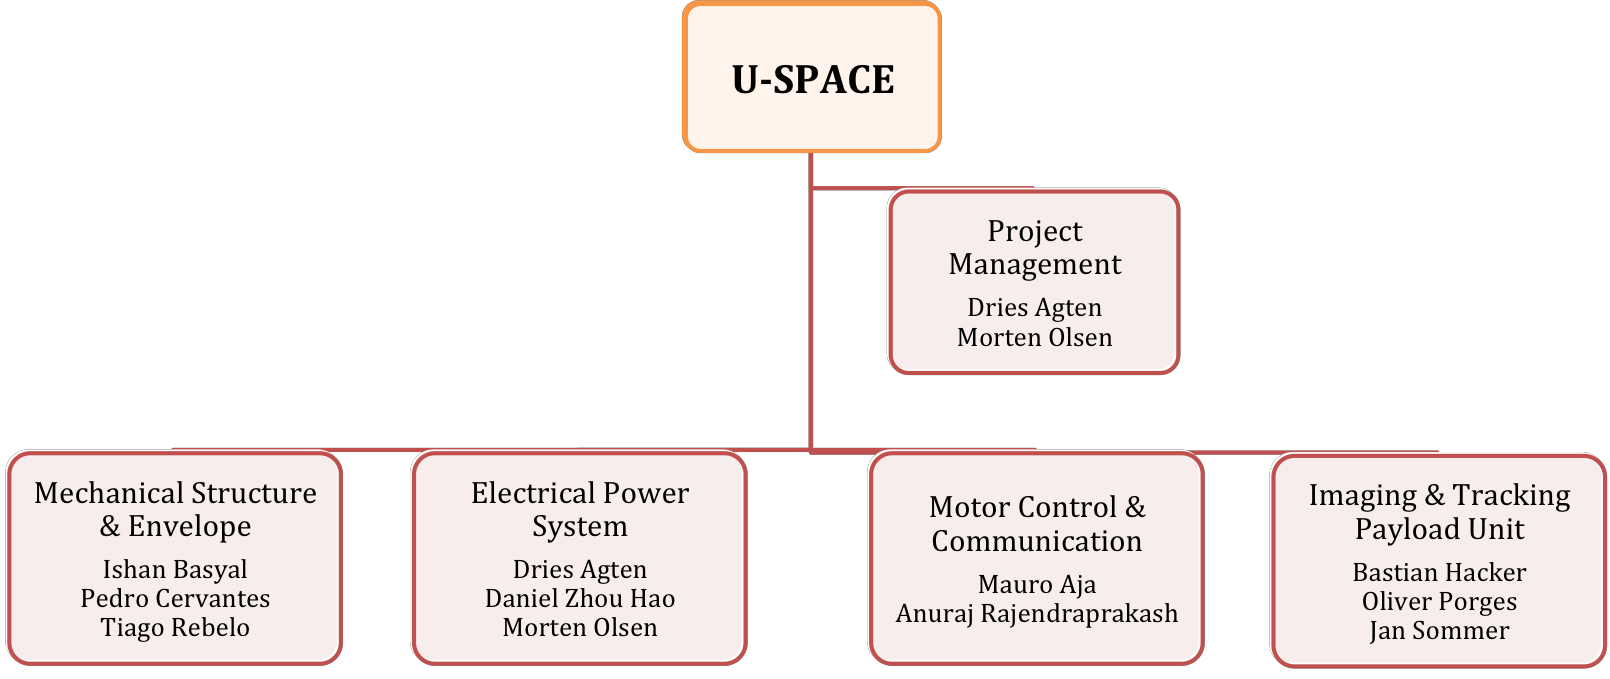
\includegraphics[width = \textwidth]{figures/obs.png} %scale=0.5
\caption{Functional organigram}
\label{fig:obs}
\end{figure}
%
\begin{table}[h]
\centering
\caption{Background of team members}
\begin{tabular}{l l}
\hline
\textbf{Name} & \textbf{Background} \\
\hline
Dries Agten & M.Sc. Eng. - Nanoscience \& Nanotechnology \\
Mauro Aja & B.Sc. Eng. - Electronic and Computer Engineering \\
Ishan Basyal & B.Sc. Earth and Space Sciences  \\
Pedro Cervantes & B.Sc. Eng. - Aeronautical Engineering \\
Bastian Hacker & B.Sc. Physics\\
Daniel Zhou Hao & B.Sc. Eng. - Aerospace Engineering\\
Morten Olsen & B.Sc. Eng. - Electrical Engineering \\
Oliver Porges & B.Sc. Cybernetics and Measurement  \\
Anuraj Rajendraprakash & B.Tech. Electronics Engineering \\
Tiago Rebelo & B.Sc. Eng. - Aeronautical Engineering \\
Jan Sommer & B.Sc. Computational Science \\
\hline
\end{tabular}
\label{tab:backgrounds}
\end{table}
%
\subsection{Support Facilities}
%
The support facilities of the \ac{U-SPACE} project are the responsibility of three organisations, each with a focus on a specific part of the project. The first organisation is \ac{LTU}, represented by Alf Wikström. As all team members are students from \ac{LTU}, this university is the principal support facility during the \ac{U-SPACE} project. Its responsibility is the practical, financial and also technical support of the team members. The practical support consists of providing tools and specific work spaces, such as mechanical workshops or electronics laboratories. Some other aspects are discussed in more detail in section \ref{sec:relation_support}.
\\
\\
The two other supporting organisations are \ac{IRF} and Esrange. \ac{IRF} is represented by Kjell Lundin, while the contacts with Esrange are the responsibility of Alf Wikström. These two support facilities provide technical assistance during the course of the project, consisting of guidance regarding the selection of the components, support during the fabrication procedures and recommendations regarding the test set-up.
%
\subsection{Transport}
%
The transportation of the prototype \ac{SPA} is an important topic in this project. Since the prototype will be built at the Rymdcampus of \ac{LTU} and since the test flight will most probably take place at Esrange, a secure transport procedure has to be developed. As the envelope is the property of Esrange (see chapter \ref{chap:mse}), the complete assembly of the airship will only take place at this location, which relieves the transport constraints. Most subsystem are limited in size and can easily be  transported in a normal passenger car. The only exception is the solar array and supporting mechanical structure which might be difficult to fit inside a car. A closed trailer or small truck might be needed for transportation of this.
%
%
\section{Relation With Support Facilities}
\label{sec:relation_support}
%
The support facilities mentioned in the previous section play an important role in the course of the \ac{U-SPACE} project. Their responsibilities are wide, ranging from reports over components to finances.
%
\subsection{Reporting and Monitoring}
%
During the entire project the team is monitored by the supervisors Kjell Lundin (\ac{IRF}) and Alf Wikström (\ac{LTU}). This monitoring task consists of controlling the budget, approving the ordering of components and evaluating the (technical) progress of the team at strategical points in time. Weekly meetings between the two supervisors and the two team managers are scheduled to identify, discuss and solve all issues that have come up since the last meeting. Apart from these weekly meetings, communication via email and telephone is used to keep the supervisors updated about the status of the project and to ask for assistance when needed.
%
\subsection{Reviews}
%
Three main reviews are planned for the \ac{U-SPACE} project:
%
\begin{itemize}
\item \acl{PDR}
\item \acl{CDR}
\item \acl{FRR}
\end{itemize}
%
The first two reviews are also the points in time when grades are connected to the work executed up to those points. Each review is briefly described below.
%
\subsubsection*{\acl{PDR}}
The \ac{PDR} was held and approved in early April 2012. With the help of five separate documents, the general project and the different subsystems were introduced to the supervisors, with a focus on the preliminary design concepts. The supervisors approval of the \ac{PDR} made the project budget available and allowed the first components to be ordered.
%
\subsubsection*{\acl{CDR}}
In the \ac{CDR}, which is the current document, the final designs of the subsystems are presented, together with some early verification and prototype results. An oral team presentation was held already in the middle of June 2012, before many team members had to leave Kiruna. The outcome of the \ac{CDR} is to ensure that the complete system design will meet the functional requirements from Section \ref{chap:goals_constraints} and the technical requirements stated for each subsystem. It must also show that all the system interfaces between different subsystems or the environment are compatible.
%
\subsubsection*{\acl{FRR}}
A third optional \ac{FRR} is also planned. This is to be held prior to flight, to ensure that all systems are fully functional and inter-compatible with each other and that all support equipment needed for a successful flight are available. This review is important since flight events at Esrange are expensive and the availability of the Esrange facilities and help from the staff is limited.
%
%
\subsection{Component Ordering}
%
The ordering of the components is the responsibility of \ac{LTU}, the organization that is also responsible for the project financing (see section \ref{sec:financing}). The members of the subsystems select the appropriate components and pass the order on to the project manager. He consults with the project supervisors and after approval the components are ordered, usually by Lars Jakobsson(LTU). Components are preferably ordered from inside Sweden, but international orders have also been possible.
%
\section{Financing}
\label{sec:financing}
%
The \ac{U-SPACE} project is financed by \ac{LTU}, the principal support facility. For each European team member, the team receives 2,000 SEK, amounting for a total budget of 14,000 SEK. This budget has to be used for the ordering of all components and for any other expenses that might arise during the course of the project (e.g. tools). An increase in the budget can be realized after an application procedure and approval by \ac{LTU}. As of this writing, the \ac{U-SPACE} project still has 4,824 SEK left of its initial budget. As was mentioned in Table \ref{tab:expected_performance}, a request for more funds for \ac{EPS} is under preparation.
%
%
\section{Schedule and Milestones}
%
Since the \ac{U-SPACE} project is a student project that has to be realized within a limited amount of time a tight schedule and a clear definition of important milestones are vital for the success of the project. The schedule has to updated regularly to reflect the current progress and/or delays of the project. The most recent schedule is shown in figure \ref{fig:schedule} below. All important milestones and test programs are indicated as well.
%
\begin{sidewaysfigure}
\centering
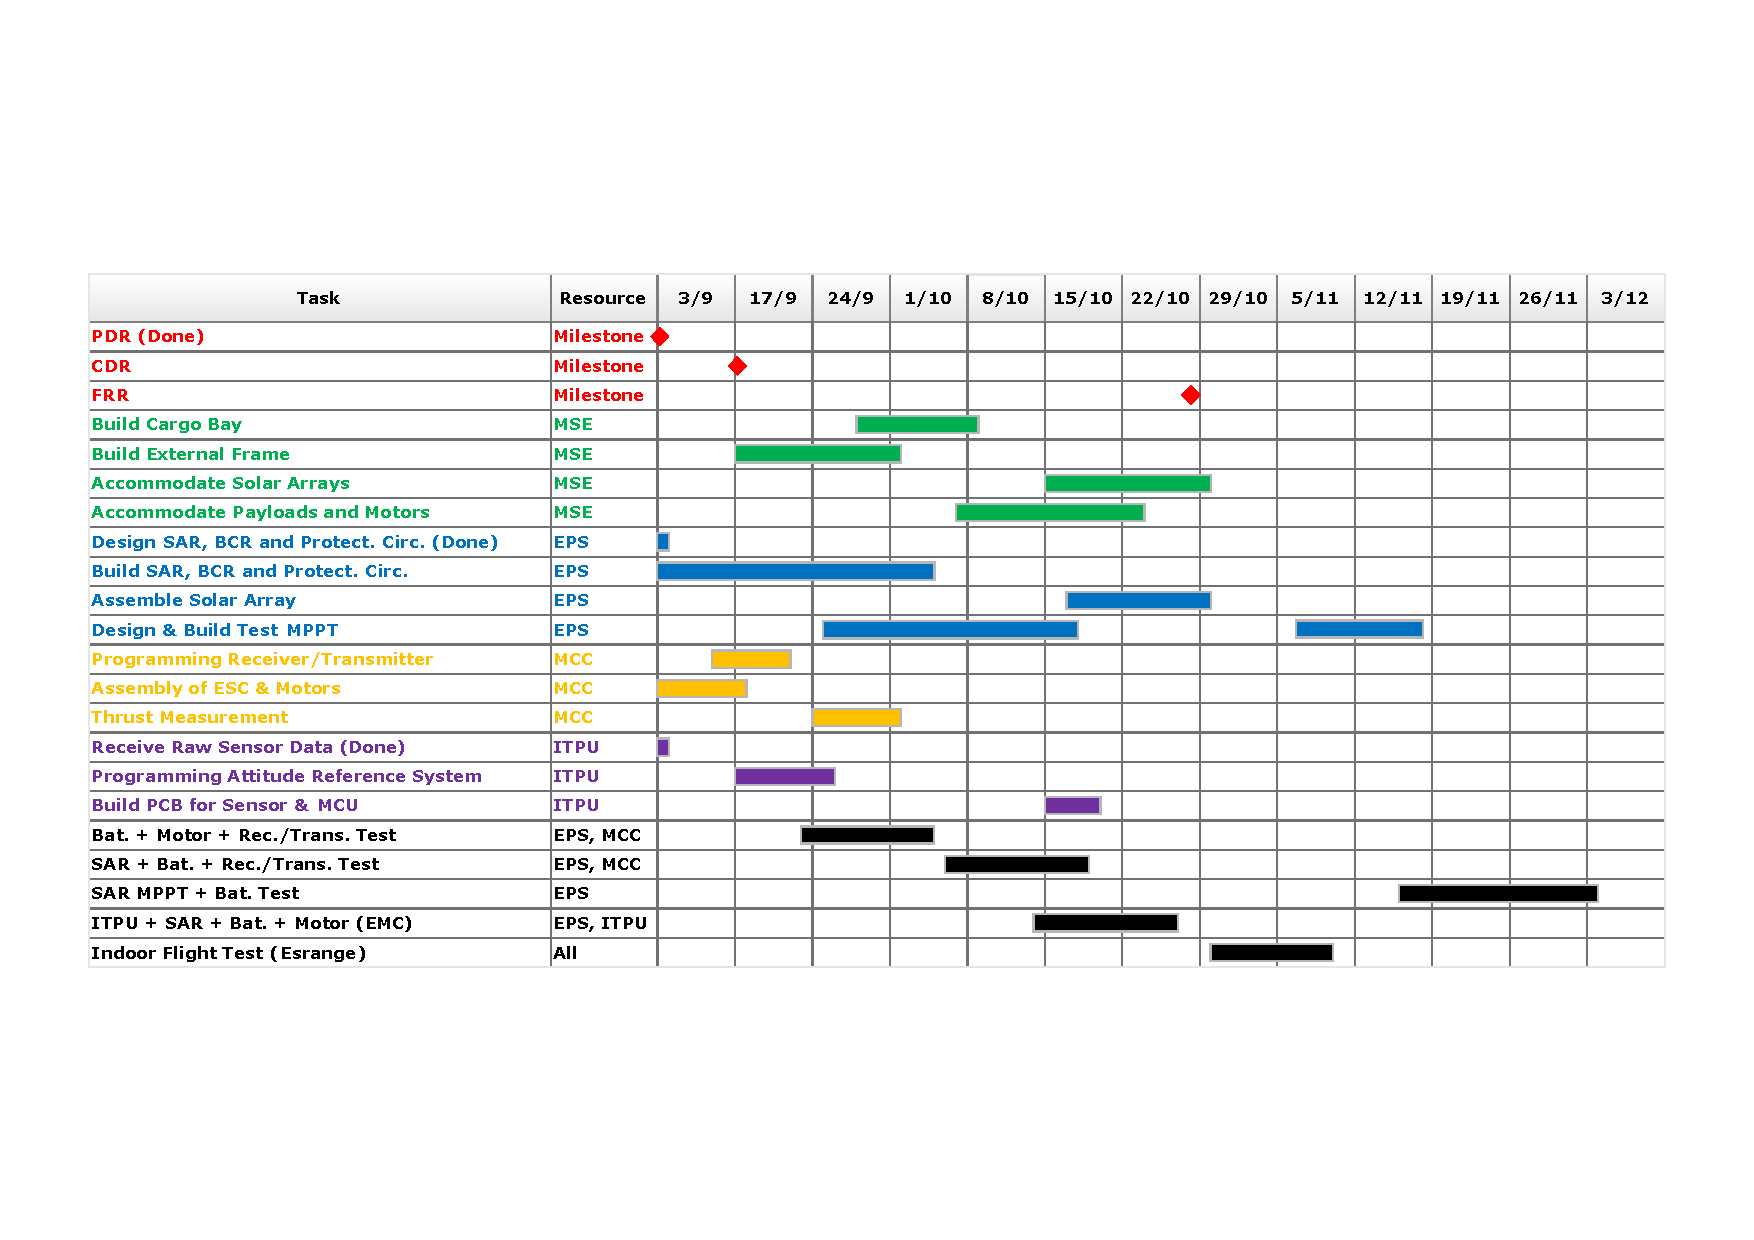
\includegraphics[width=\textwidth]{figures/fig_CDR_PM_GanttChart}
\caption{Project Plan}
\label{fig:project_plan}
\end{sidewaysfigure}
%
%
\section{Configuration Control}
%
Although the \ac{U-SPACE} project is limited in size, configuration control remains an important element of the success of the project. With four different subsystems and many different team members it is essential to have a common platform where design changes are listed, tracked and discussed. This is necessary to guarantee technical consistency and to avoid misunderstandings that may endanger the outcome of the project.
\\
\\
The main component of the \ac{U-SPACE} configuration control is a weekly meeting of all team members. An agenda is composed beforehand by the meeting chair, listing all important issues, both practical and technical, that have to be discussed during the meeting. A meeting secretary is responsible for producing minutes of the meeting. These minutes, together with the agendas, are accessible for the entire team by the use of Google Docs. Another minor component of the configuration control is the revision control system GitHub, which is mainly used to share the documents that make up the design review. It is also the place where the developed \ac{ITPU} code is made available to the relevant team members. For minor issues, emails to a common team email address are used.
%
\section{Deliverables}
%
The ultimate goal of the \ac{U-SPACE} project is to realize a functioning prototype of a \ac{SPA} capable of forward propulsion while supporting a scientific payload. Since this project is a student project under the supervision of \ac{LTU}, the final phases of the project also require the handing in of several deliverables.
%
\subsection{Hardware and Software}
%
The main deliverable is a functioning prototype of an \ac{SPA}, consisting of several separately developed subsystems (see chapters \ref{chap:mse} through \ref{chap:itpu}). Each subsystem should function on its own as well as in concurrence with the other subsystems. All necessary components have to be included when the subsystem is delivered.
\\
\\
Also the ground station is a deliverable, although it is mainly software-based. All code has to be delivered at the end of the project, together with comments that explain the code (see the following subsection). Also the code written for the airborne part of the \ac{ITPU} has to be included.
%
\subsection{Documentation}
%
The deliverable documentation first of all consists of both design reviews (\ac{PDR} and \ac{CDR}), which are documents that provide details on the functioning of each subsystem and on the general elements of the project. When available, all documents that were used during the development of a subsystem should be classified and stored for future use. This allows future team members to easily pick up the work where it was left by their predecessors.
\\
\\
Apart from these hardware-related documents, documentation regarding the developed software should also be delivered. This documentation mainly consists of comments on the code such that it may be understood and further developed by future team members.